% Quiz 08 --- answer key with marking notes. DO NOT HAND OUT.
%
% Every number was checked with numpy: the 25-node 5 x 5 grid Laplacian Lx,
% the 8-node double-diamond spectrum and Fiedler vector u, every single-edge
% removal, and every single-edge addition.
%
% Compile with: xelatex -interaction=nonstopmode solutions.tex   (run twice)
\documentclass[a4paper, 11pt]{extarticle}
% Shared preamble for Quiz 08 (quiz08.tex and solutions.tex).
% Compile with: xelatex -interaction=nonstopmode <file>.tex   (run twice)
%
% Same house look as the pen-and-paper sheets in
% lecture-note/*/pen-and-paper/: Charter, A4, generous leading, room to draw.

\usepackage[top=0.7in, bottom=0.6in, left=0.8in, right=0.8in]{geometry}
\usepackage{amsmath}
\usepackage{amssymb}
\usepackage{array}
\usepackage{graphicx}
\usepackage[hidelinks]{hyperref}
\usepackage{tcolorbox}
\usepackage{enumitem}
\usepackage{etoolbox}
\usepackage{tikz}
\usepackage{fontspec}
\usetikzlibrary{calc,positioning,arrows.meta}
\definecolor{pltblue}{HTML}{1F77B4}
\definecolor{rulegrey}{HTML}{6A6D75}

% Body face. Charter, and the four ways to get it. XCharter *is* Charter and
% ships with a full TeX Live, so it is asked for first and by file: a CI runner
% answers yes to \IfFontExistsTF{Charter}, then cannot typeset it.
\IfFontExistsTF{XCharter-Roman.otf}{
  \setmainfont{XCharter}[
    Extension      = .otf,
    UprightFont    = *-Roman,
    BoldFont       = *-Bold,
    ItalicFont     = *-Italic,
    BoldItalicFont = *-BoldItalic]
}{
  \IfFontExistsTF{Charter}{\setmainfont{Charter}}{
    \IfFontExistsTF{Iowan Old Style}{\setmainfont{Iowan Old Style}}{
      \IfFontExistsTF{Georgia}{\setmainfont{Georgia}}{}}}}

\setlength{\parindent}{0pt}
\setlength{\parskip}{0.4em}
\setlength{\emergencystretch}{1.2em}
\raggedbottom
\pagestyle{empty}

% ---------------------------------------------------------------------------
% The submission link.
%
% Both the QR square and the printed address are the course's own short link,
% not the form's: paper outlives any one form. Caddy on the course droplet
% points go.skojaku.com/ans-quiz08 at the current Google Form
% (/etc/caddy/Caddyfile, block go.skojaku.com). Swapping the form is a line on
% the server, not a reprint.
%
% If the link ever changes, rebuild the square with
%
%   uvx --from segno segno --output=quiz08-form-qr.png --scale=20 --border=1 \
%       --error=m "<the url>"
% ---------------------------------------------------------------------------
\newcommand{\formlink}{https://go.skojaku.com/ans-quiz08}
\newcommand{\formshort}{\href{\formlink}{\texttt{go.skojaku.com/ans-quiz08}}}

% Quiz header. #1 = title, #2 = the line under it, #3 = term.
\newcommand{\quizhead}[3]{%
  {\footnotesize\textsc{Advanced Network Science} \hfill \textsc{#3}}\par
  \vspace{-0.2em}\rule{\textwidth}{1pt}\par
  \vspace{0.3em}
  {\LARGE\bfseries #1}\par
  \vspace{0.1em}
  {\small #2}\par
  \vspace{0.7em}
  {\small Name \underline{\hspace{6cm}} \hfill Date \underline{\hspace{3.2cm}}}\par
  \vspace{0.7em}}

% A question heading with its point value.
\newcommand{\question}[3]{%
  \vspace{0.5em}
  {\large\bfseries Question #1 \quad\normalsize\mdseries (#2 points)}\par
  \vspace{-0.3em}{\color{rulegrey}\rule{\textwidth}{0.6pt}}\par
  \vspace{0.1em}
  {\bfseries #3}\par
  \vspace{0.2em}}

% An empty box to draw or write in. #1 = height, #2 = caption under the rule.
\newcommand{\drawbox}[2]{%
  \begin{tcolorbox}[colback=white, colframe=rulegrey, boxrule=0.5pt,
                    sharp corners, height=#1, valign=top,
                    boxsep=2pt, left=4pt, right=4pt, top=3pt, bottom=3pt]
  {\footnotesize\color{rulegrey} #2}
  \end{tcolorbox}}

% Ruled writing lines, #1 of them.
\newcommand{\writelines}[1]{%
  \vspace{0.3em}
  \foreach \i in {1,...,#1}{%
    {\color{rulegrey}\rule{\textwidth}{0.4pt}}\par\vspace{1.5em}}}

\newgeometry{top=0.4in, bottom=0.4in, left=0.75in, right=0.75in}
\setlength{\parskip}{0.28em}

\renewcommand{\question}[3]{\vspace{0.25em}
  {\large\bfseries Question #1 \quad\normalsize\mdseries (#2 points) --- #3}\par
  \vspace{-0.3em}{\color{rulegrey}\rule{\textwidth}{0.6pt}}\par\vspace{0.1em}}
\newcommand{\ans}[1]{{\color{pltblue}#1}}

\begin{document}
\small

\quizhead{Quiz 8 \; --- \; Answer key}
        {Instructor copy \quad$\cdot$\quad do not hand out}
        {Fall 2026}

% ---------------------------------------------------------------------------
\question{1}{5}{What does the Laplacian do to an image?}

\textbf{(a) [1]} Since $D_{ii} = k_i = |\mathcal{N}(i)|$ and $A_{ij} = 1$ iff $j \in \mathcal{N}(i)$,
\[
  (Lx)_i \;=\; (Dx - Ax)_i \;=\; k_i x_i - \sum_{j \in \mathcal{N}(i)} x_j
  \;=\; \ans{\sum_{j \in \mathcal{N}(i)} (x_i - x_j)} .
\]

\begin{minipage}[c]{0.66\textwidth}
\textbf{(b) [2]} Evaluating $(Lx)_i = \sum_{j \in \mathcal{N}(i)}(x_i - x_j)$ on the 4-neighbor grid gives the table on the right (border pixels have degree 2 or 3, and the formula uses only existing neighbors).

\smallskip
\textbf{Marks for (b) [2]:} Full marks (2) for all 25 entries right (if a student defines $A - D$ consistently and flips every sign, deduct 0.5). Deduct 1 if border pixels are treated as degree 4 instead of 2 or 3, or if square corners are written as $+1$ instead of $+2$.
\end{minipage}
\hfill
\begin{minipage}[c]{0.31\textwidth}
\centering
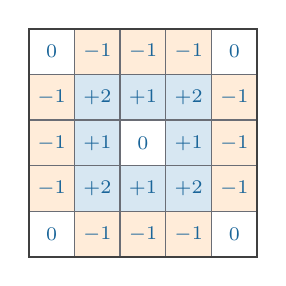
\begin{tikzpicture}[x=0.58cm, y=0.58cm]
  \foreach \row [count=\r from 0] in {
    {0,-1,-1,-1,0},
    {-1,+2,+1,+2,-1},
    {-1,+1,0,+1,-1},
    {-1,+2,+1,+2,-1},
    {0,-1,-1,-1,0}} {
    \foreach \v [count=\c from 0] in \row {
      \ifnum\v>0
        \fill[pltblue!18] (\c, 4-\r) rectangle (\c+1, 5-\r);
      \fi
      \ifnum\v<0
        \fill[orange!15] (\c, 4-\r) rectangle (\c+1, 5-\r);
      \fi
      \node[font=\scriptsize\bfseries, text=pltblue!85!black] at (\c+0.5, 4.5-\r) {$\v$};
    }
  }
  \foreach \i in {1,...,4} {
    \draw[rulegrey, line width=0.5pt] (\i,0) -- (\i,5);
    \draw[rulegrey, line width=0.5pt] (0,\i) -- (5,\i);
  }
  \draw[black!75, line width=0.8pt] (0,0) rectangle (5,5);
\end{tikzpicture}
\end{minipage}

\smallskip
\textbf{(c) [2]} Multiplying by $L$ acts as an \ans{edge / boundary detector} (1 pt): it highlights where pixel values change abruptly (positive inside the rim, negative outside, largest at the four corners where two neighbors differ) while zeroing out uniform regions. The center pixel gives \ans{$0$ because all four of its neighbors also have $x_j = 1$}, so every difference $x_i - x_j = 0$ (1 pt): $L$ measures \emph{local contrast with neighbors}, not raw brightness.

\textbf{Not asked, for the lecturer.} $\sum_i (Lx)_i = \mathbf{1}^\top L x = 0$ ($+12$ inside cancels $-12$ outside), and $x^\top L x = 12$ is the exact perimeter (cut size) of the $3\times 3$ square.

% ---------------------------------------------------------------------------
\question{2}{5}{Network surgery.}

Eigenvalues of $L$: $0,\ 0.2907,\ 2,\ 2.8061,\ 4,\ 4,\ 4,\ 4.9032$. Every node has degree $\ge 2$ (no leaves), so D--E is the \emph{unique} bridge.
Exact Fiedler vector: $u = (-0.4325,\allowbreak -0.3696,\allowbreak -0.3696,\allowbreak -0.1993,\allowbreak +0.1993,\allowbreak +0.3696,\allowbreak +0.3696,\allowbreak +0.4325)^\top$.

\textbf{(a) [2]} Cut edge \ans{D--E} (1 pt). How $u$ identifies it (1 pt):
(i) D--E is the \emph{only} edge whose endpoints have opposite signs in $u$ ($-0.20$ vs.\ $+0.20$), so it is the sole edge crossing the Fiedler bipartition $\{A,B,C,D\} \mid \{E,F,G,H\}$; and
(ii) it has the largest difference $|u_i - u_j| = 0.40$ among all existing edges, contributing $(u_D - u_E)^2 = 0.159$ (over half of $\lambda_2 = 0.291$). Either observation clearly stated earns the explanation point.

\textbf{(b) [3]} Connect \ans{A and H} (1 pt). Adding edge $(i,j)$ changes $L$ to $L' = L + L_{ij}$, adding one new spring term $(u_i - u_j)^2$ to the quadratic form:
\[
  u^\top L' u \;=\; u^\top L u + (u_i - u_j)^2 \;=\; \lambda_2 + (u_i - u_j)^2 .
\]
(By first-order perturbation of a simple eigenvalue, $\Delta\lambda_2 \approx (u_i - u_j)^2$.) To raise $\lambda_2$ as much as possible, maximize $(u_i - u_j)^2$ by connecting the two nodes with the largest gap $|u_i - u_j|$: the most negative node A ($-0.43$) and the most positive node H ($+0.43$), giving $|u_A - u_H| = 0.86$ and $(u_A - u_H)^2 \approx 0.75$.

\textbf{Marks for (b) [3]:} Naming A--H (1); showing that adding $(i,j)$ adds $(u_i - u_j)^2$ to $u^\top L u$ (1); concluding that we maximize $|u_i - u_j|$, picking the two opposite extremes rather than nodes near the bridge or degree-3 hubs (1).

\smallskip
\textbf{Exact check across candidate additions (for the lecturer):}
\vspace{-0.3em}
\begin{center}
\footnotesize
\begin{tabular}{lccc}
\hline
Added edge & $|u_i - u_j|$ & $(u_i - u_j)^2$ & Exact new $\lambda_2$ (was $0.291$) \\
\hline
\textbf{A--H} (opposite extremes) & $0.865$ & $0.748$ & \textbf{$0.764$} \\
A--F, A--G, B--H, C--H & $0.802$ & $0.643$ & $0.707$ \\
B--F, B--G, C--F, C--G (degree-3 hubs) & $0.739$ & $0.547$ & $0.668$ \\
B--E, C--E, D--F, D--G (near bridge) & $0.569$ & $0.324$ & $0.491$ \\
A--D, E--H (same side) & $0.233$ & $0.054$ & $0.319$ \\
\hline
\end{tabular}
\end{center}
\vspace{-0.3em}
\textbf{Not asked, for the lecturer.} The vertical diagonals B--C ($u_B = u_C = -0.37$) and F--G ($u_F = u_G = +0.37$) have $(u_i - u_j)^2 = 0$: cutting either leaves $\lambda_2 = 0.2907$ completely unchanged.

\end{document}
